\documentclass[12pt]{article}
\usepackage[utf8]{inputenc}
\usepackage[a4paper, margin=2cm]{geometry}
\usepackage[T1]{fontenc}
\usepackage{graphicx}
\usepackage{geometry}
\usepackage{amsmath}
\usepackage{amsfonts}
\usepackage{amssymb}
\usepackage{booktabs}
\usepackage{hyperref}
\usepackage{fancyhdr}
\usepackage{float}
\usepackage{ulem}
\usepackage{xeCJK}
\usepackage{listings}
\usepackage{xcolor}
\usepackage{indentfirst}
\setmainfont{Times New Roman}
\setCJKmonofont[BoldFont=SimHei, AutoFakeBold=true]{SimSun}
\lstset{
    basicstyle=\ttfamily\small,
    commentstyle=\color{gray},
    keywordstyle=\color{blue},
    stringstyle=\color{red},
    numberstyle=\tiny\color{gray},
    breaklines=true,
    captionpos=b,
    keepspaces=true,
    numbers=left,
    numbersep=5pt,
    showspaces=false,
    showstringspaces=false,
    showtabs=false,
    tabsize=2,
    frame=single,
    language=[x86masm]Assembler
}

\begin{document}
\thispagestyle{empty}

\begin{center}
    \vspace*{2cm}
    
    \Huge \textbf{2023-2024学年春季学期} \\
    \vspace{2cm}
    
    \Huge \textbf{《汇编语言程序设计》} \\
    \vspace{4cm}
    
    \large 评分：\underline{\hspace{4cm}} \\
    \vspace{6cm}
    
    \begin{tabular}{rl}
        \Large 学\hspace{2em}院： & \Large \underline{\makebox[12em][l]{\quad 计算机科学与工程学院}} \\
        \Large 专\hspace{2em}业： & \Large \underline{\makebox[12em][l]{\quad 计算机科学与技术}} \\
        \Large 班\hspace{2em}级： & \Large \underline{\makebox[12em][l]{\quad 计算机2204班}} \\
        \Large 姓\hspace{2em}名： & \Large \underline{\makebox[12em][l]{\quad 李俊洁}} \\
        \Large 学\hspace{2em}号： & \Large \underline{\makebox[12em][l]{\quad 20225443}} \\
        \Large 任课教师：         & \Large \underline{\makebox[12em][l]{\quad 刘思宇、柳秀梅}} \\
    \end{tabular}
    \vfill
\end{center}
\newpage

\section{实验目的}
本实验旨在通过汇编语言编程，实现文件复制的功能，从而加深对BIOS和DOS系统调用在文件操作中的应用。
实验将通过直接与操作系统的底层接口交互，来完成从一个文件到另一个文件的数据复制任务。

具体学习目标包括：
\begin{itemize}
    \item 理解BIOS与DOS中断调用的基本使用方法，尤其是文件操作相关的中断服务。
    \item 学习如何通过汇编语言进行文件的读取和写入，掌握使用系统调用处理文件的基本技巧。
    \item 掌握如何从键盘接收输入并处理字符串数据，以获取用户指定的文件名。
    \item 增强对汇编语言程序结构的理解，包括数据段和代码段的合理划分及使用。
    \item 提升程序调试和错误处理的能力，通过实际编码练习解决在文件操作中可能遇到的具体问题。
\end{itemize}

\section{实验要求}
本实验要求使用汇编语言，通过BIOS和DOS中断调用完成一个基本的文件复制程序。
需要按照下列详细要求来完成实验：

\begin{itemize}
    \item 程序必须能从键盘接收两个文件名的输入，一个作为源文件，另一个作为目标文件。
    \item 必须使用DOS中断调用来实现文件的打开、读取、写入和关闭操作。
    \item 程序应能处理不同大小的文件，保证大文件能够完整复制到目标文件中。
    \item 必须实现基本的错误处理，例如源文件不存在或目标文件无法创建时，程序应能给出相应的错误提示并安全退出。
    \item 提交的源代码必须包含详细的注释，说明每一个步骤的功能和实现方法。
    \item 实验报告中应包括程序的流程图，详细描述程序的工作流程。
    \item 实验结束后，需要记录并分析程序运行过程中出现的任何错误，提供调试过程和解决问题的详细说明。
    \item 实验报告应详细记录程序的设计思路、实现过程以及遇到的问题和解决方案。
\end{itemize}

通过完成这些要求深入理解和实践文件处理的汇编语言编程，同时也将增强处理文件输入输出和系统调用的实际应用能力。
\section{实验内容}
利用DOS的调用编程完成将一个文件复制到另一个文件中。

要求：文件名从键盘输入。
\section{源程序}
    \begin{lstlisting}[caption={汇编源代码}, label=lst:asm2]
dseg segment
    filename    db 32, 0, 32 dup(?)    ; 输入文件名缓冲区，最大长度32个字符
    errmsg      db 'File Error! $'     ; 错误信息字符串
    buff        db 255 dup(?)          ; 文件读取缓冲区，最大255个字节
    writename   db 32, 0, 32 dup(?)    ; 输出文件名缓冲区，最大长度32个字符
dseg ends

sseg segment stack 
    db 100h dup(0)
sseg ends

cseg segment
    assume cs:cseg, ds:dseg, ss:sseg
main proc far
start:
    push    ds                        ; 保存DS寄存器
    xor     ax, ax                    ; 清零AX寄存器
    push    ax                        ; 将0推入栈中，用作返回地址
    mov     ax, dseg                  ; 加载数据段地址到AX
    mov     ds, ax                    ; 设置DS寄存器
    ; 读取文件名到filename
    lea     dx, filename              ; 加载filename的地址到DX
    mov     ah, 0ah                   ; DOS中断读取字符串功能
    int     21h                       ; 调用DOS中断
    mov     dl, 0ah                   ; 输出换行符
    mov     ah, 2                     ; DOS中断显示字符功能
    int     21h                       ; 调用DOS中断
    ; 打开文件以读取
    mov     bl, filename+1
    xor     bh, bh
    mov     [bx+filename+2], bh       ; 设置字符串结束标志
    lea     dx, filename+2
    mov     ax, 3d00h                 ; DOS中断打开文件功能，模式为读取
    int     21h                       ; 调用DOS中断
    jc      return                    ; 如果出错，跳转到错误处理
    mov     bx, ax                    ; 保存文件句柄到BX
do_while:
    ; 从文件中读取数据
    mov     cx, 512                   ; 设置读取的字节数
    lea     dx, buff                  ; 设置缓冲区地址
    mov     ah, 3fh                   ; DOS中断读文件功能
    int     21h                       ; 调用DOS中断
    jc      return                    ; 如果出错，跳转到错误处理
    mov     cx, ax                    ; 保存读取的字节数到CX
    cmp     cx, 512                   ; 检查是否读满
    je      do_while                  ; 如果满，则继续读取
    mov     ah, 3eh                   ; 关闭文件
    int     21h
    ; 文件写入
    lea     dx, writename             ; 加载writename地址到DX
    mov     ah, 0ah                   ; DOS中断读取字符串功能
    int     21h                       ; 调用DOS中断
    mov     bl, writename+1
    xor     bx, bx
    mov     [bx+writename+2], bh      ; 设置字符串结束标志
    lea     dx, writename+2
    mov     ax, 3d01h                 ; DOS中断打开文件功能，模式为写入
    int     21h                       ; 调用DOS中断
    jc      return                    ; 如果出错，跳转到错误处理
    mov     bx, ax                    ; 保存文件句柄到BX
    lea     dx, buff                  ; 设置缓冲区地址
    mov     ah, 40h                   ; DOS中断写文件功能
    int     21h                       ; 调用DOS中断
    jc      return                    ; 如果出错，跳转到错误处理
    mov     ah, 3eh                   ; 关闭文件
    int     21h
    ret
return:
    ; 错误处理
    lea dx, errmsg
    mov ah, 9
    int 21h                           ; 显示错误信息
    ret
main endp

cseg ends
    end main
    \end{lstlisting}

\section{运行结果}
    \subsection{调试步骤}
    每次调试程序所输入的数据以及显示器上输出的结果:

    \begin{center}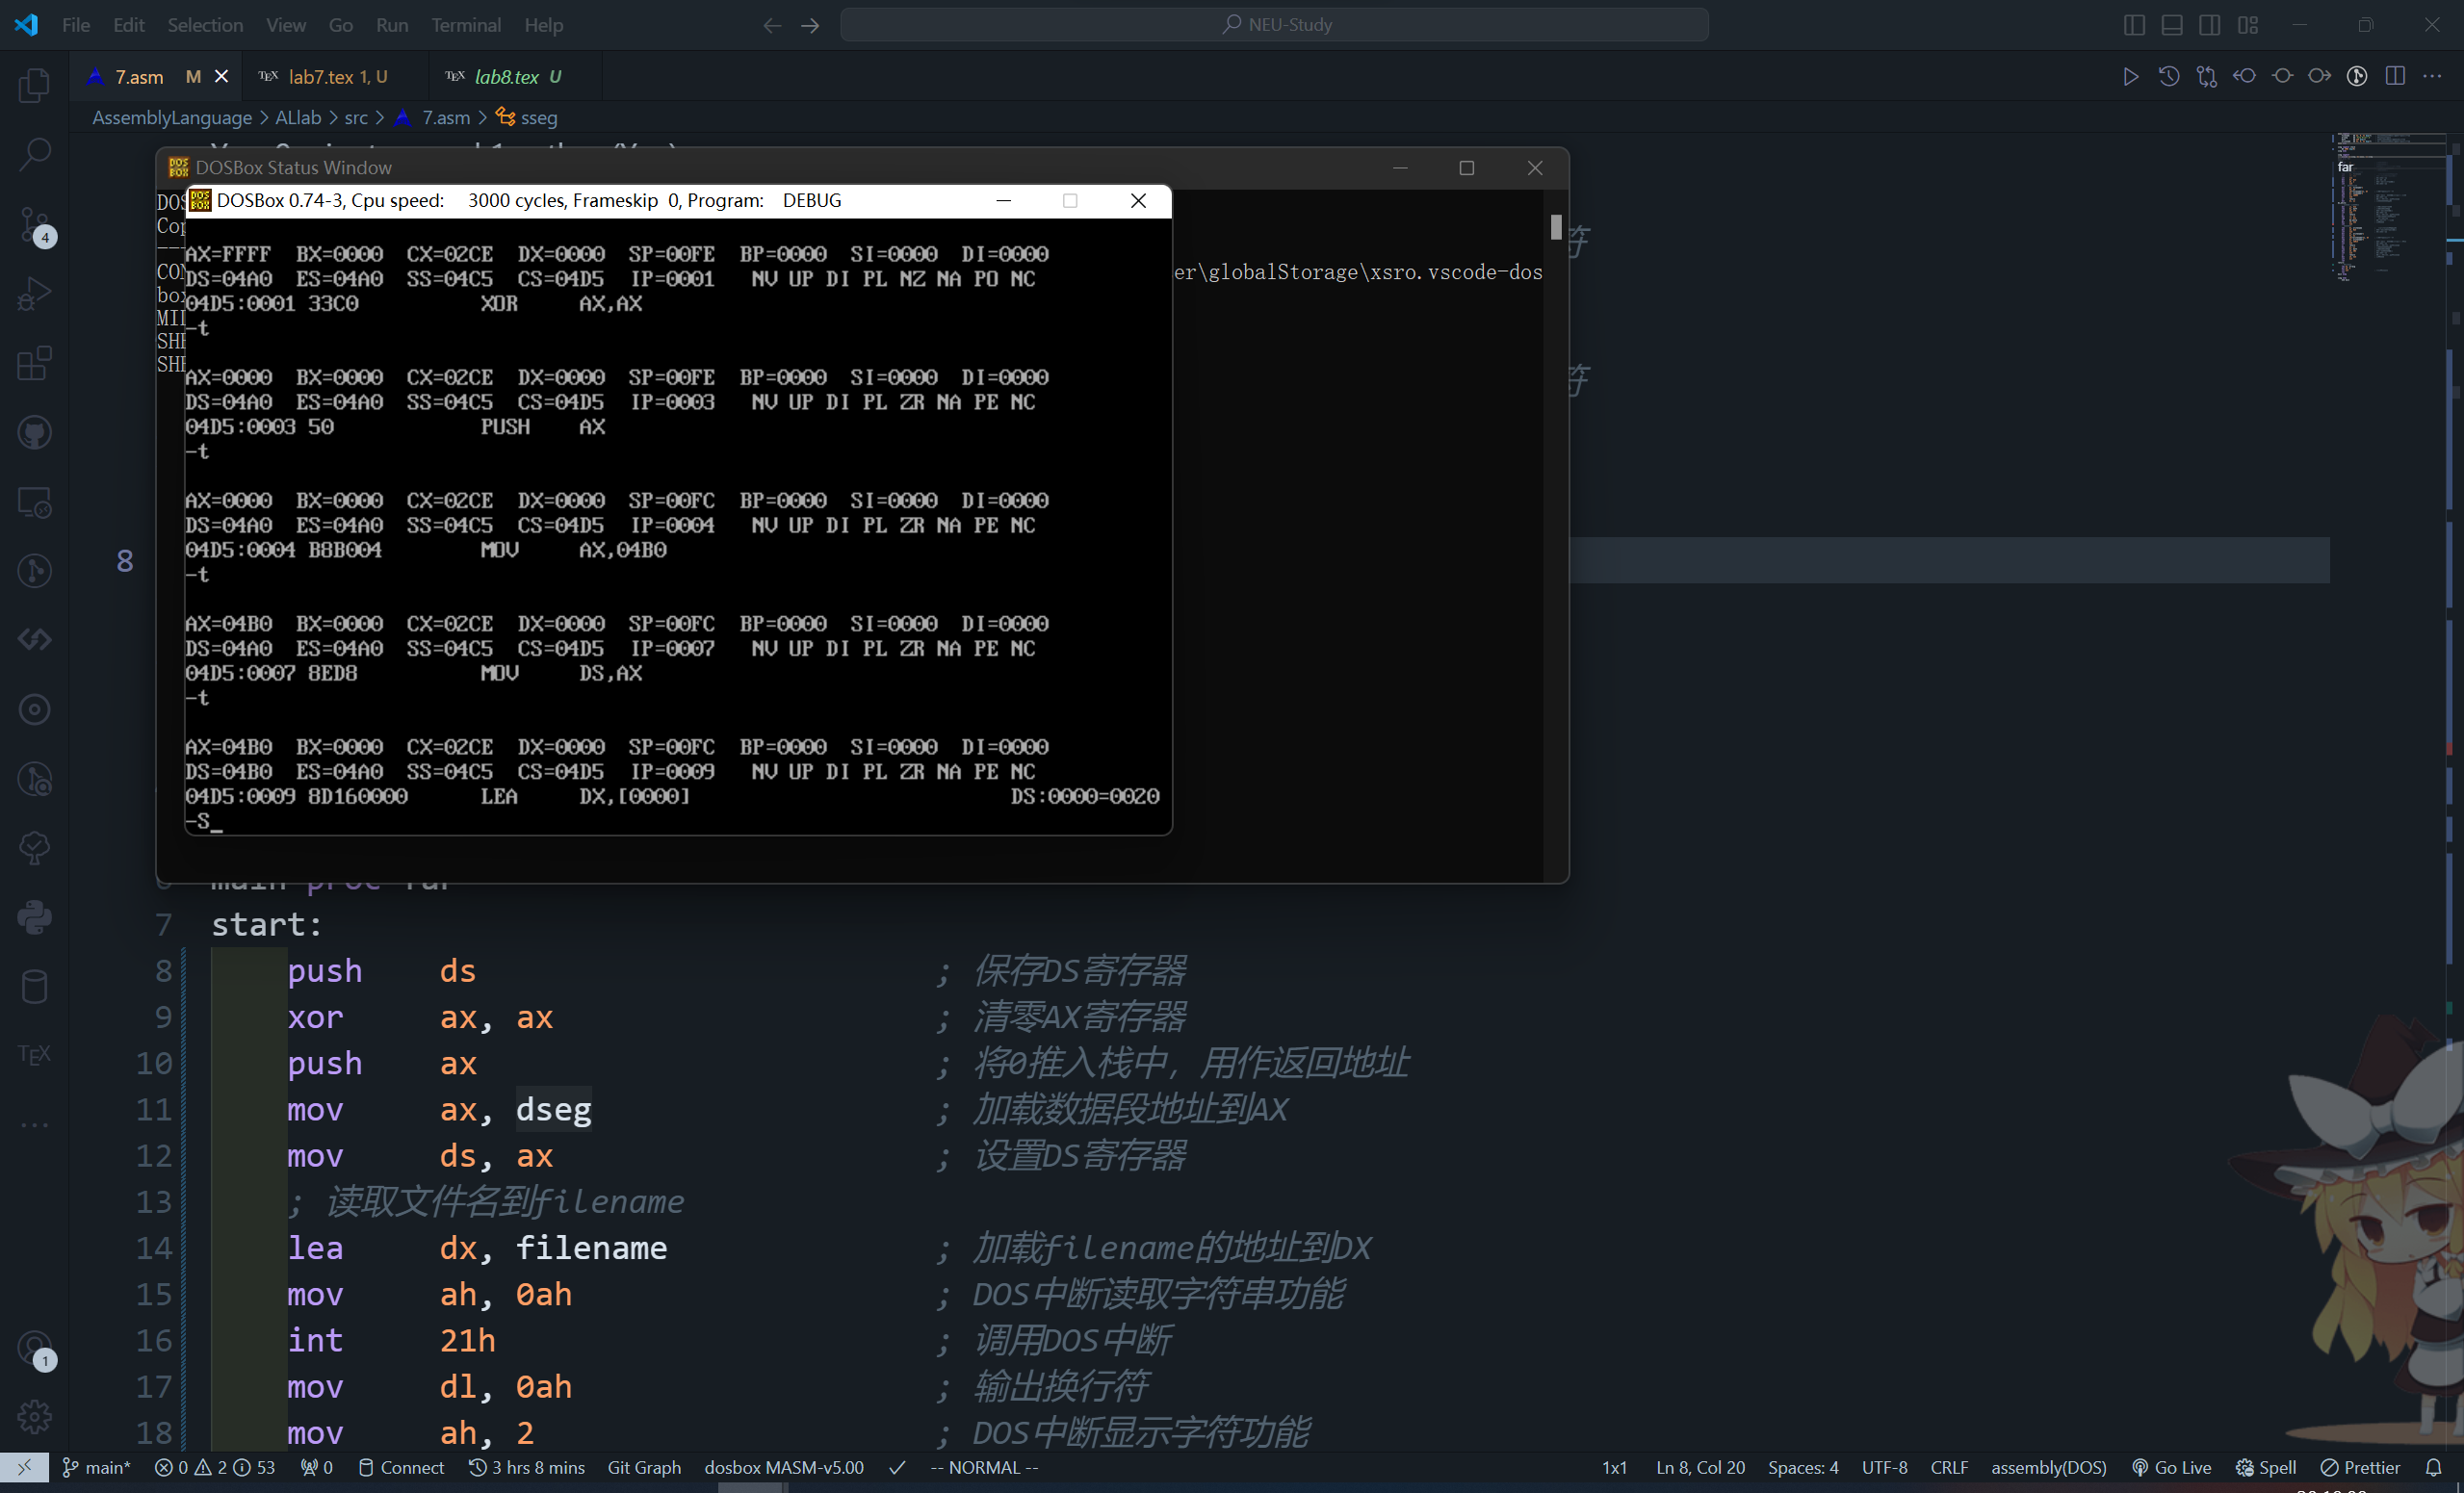
\includegraphics[width=1\textwidth]{image/AL_62.png}\end{center}
    
    错误输出：

    \begin{center}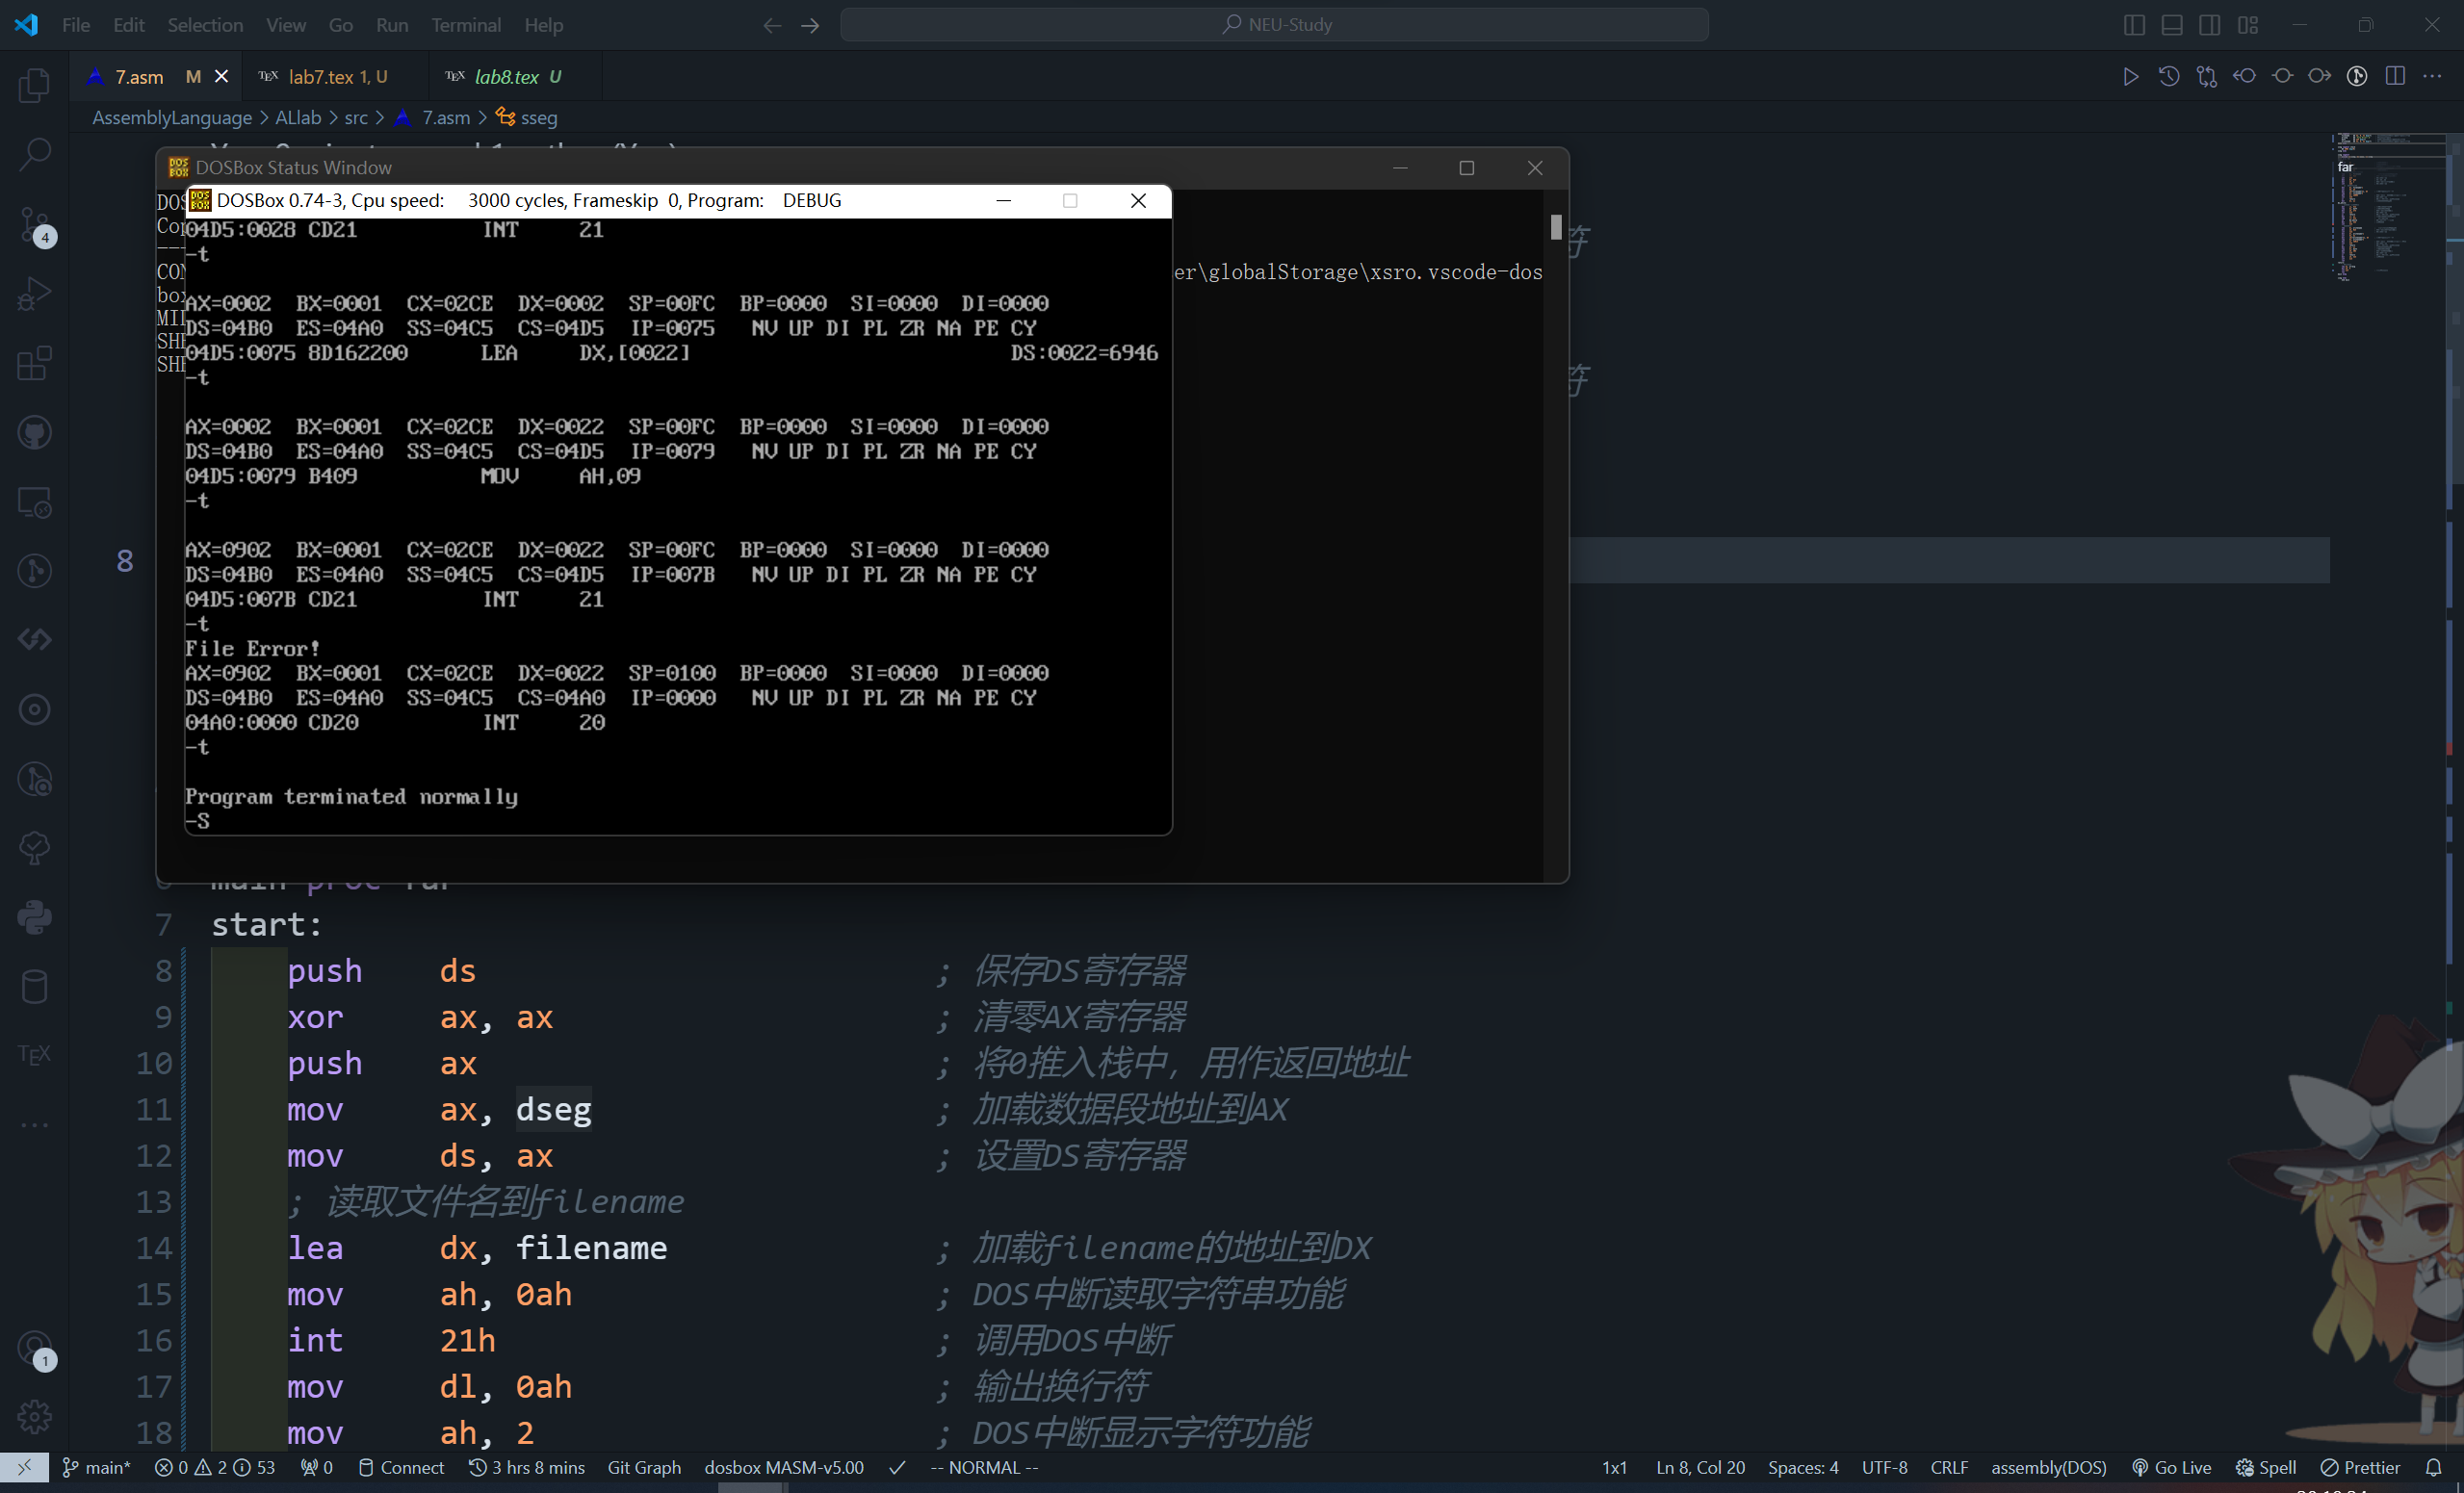
\includegraphics[width=1\textwidth]{image/AL_63.png}\end{center}

    \subsection{显示结果}
    输入文件

    \begin{center}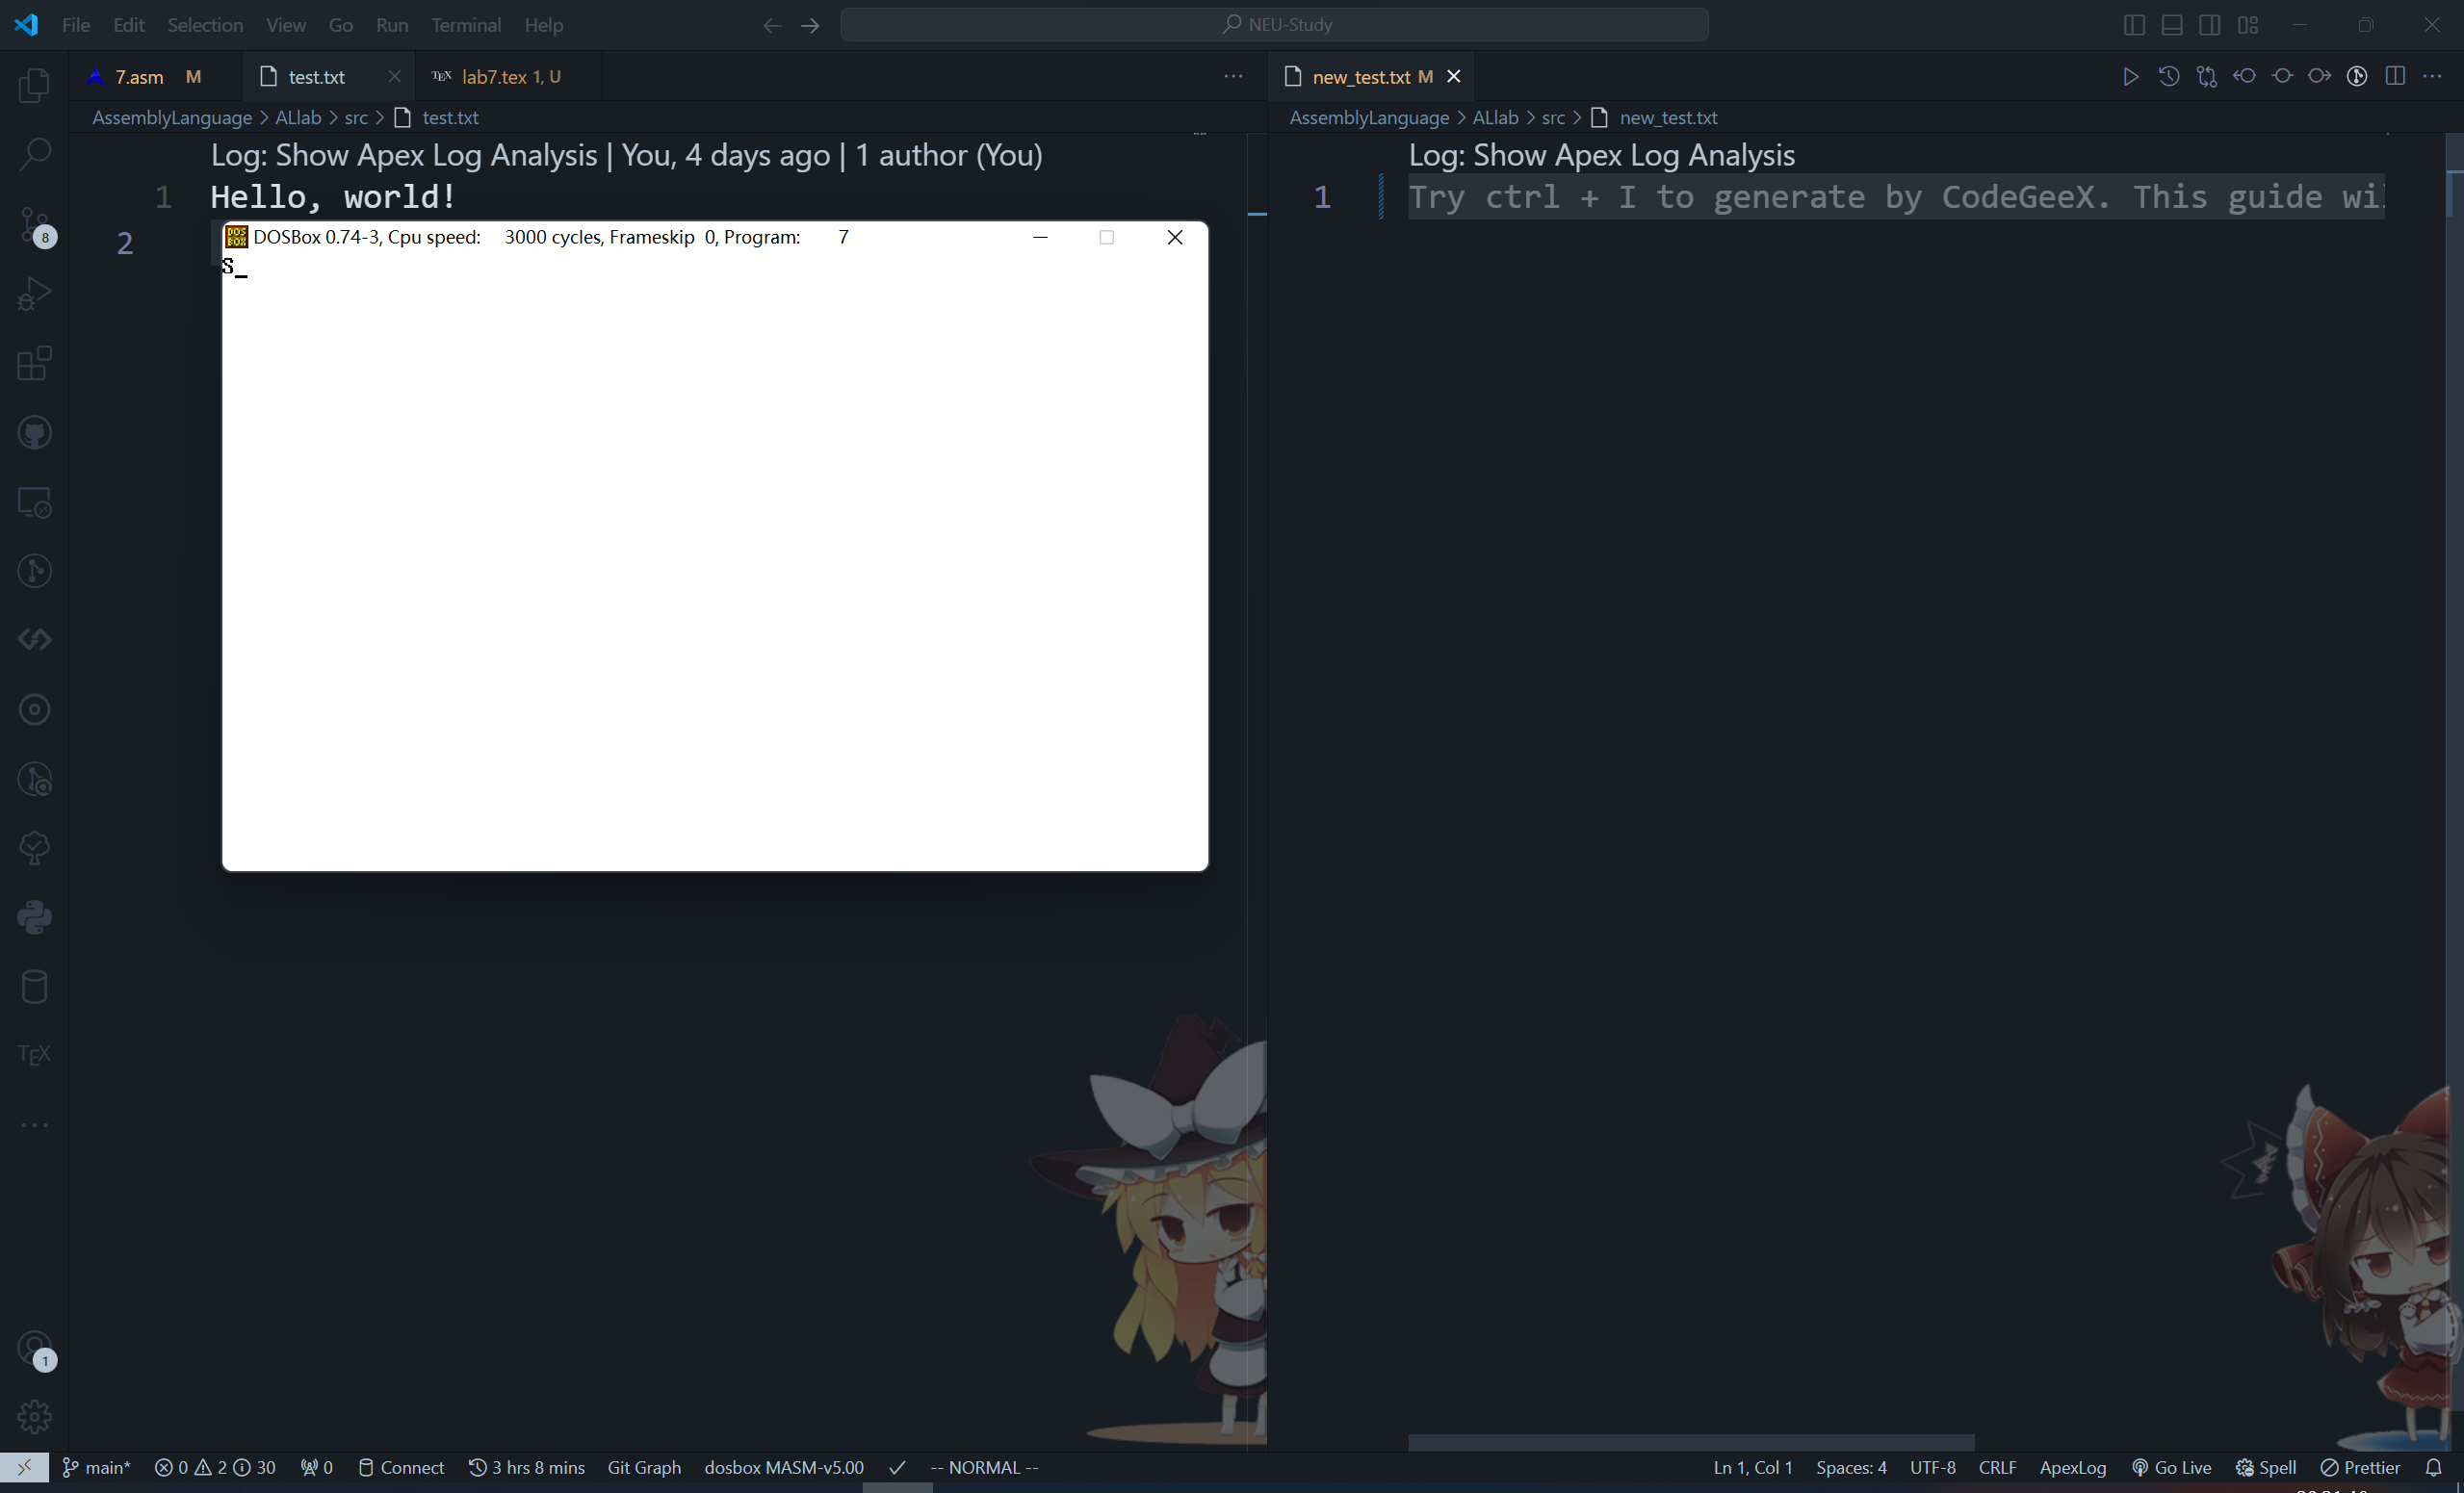
\includegraphics[width=1\textwidth]{image/AL_64.png}\end{center}
    \begin{center}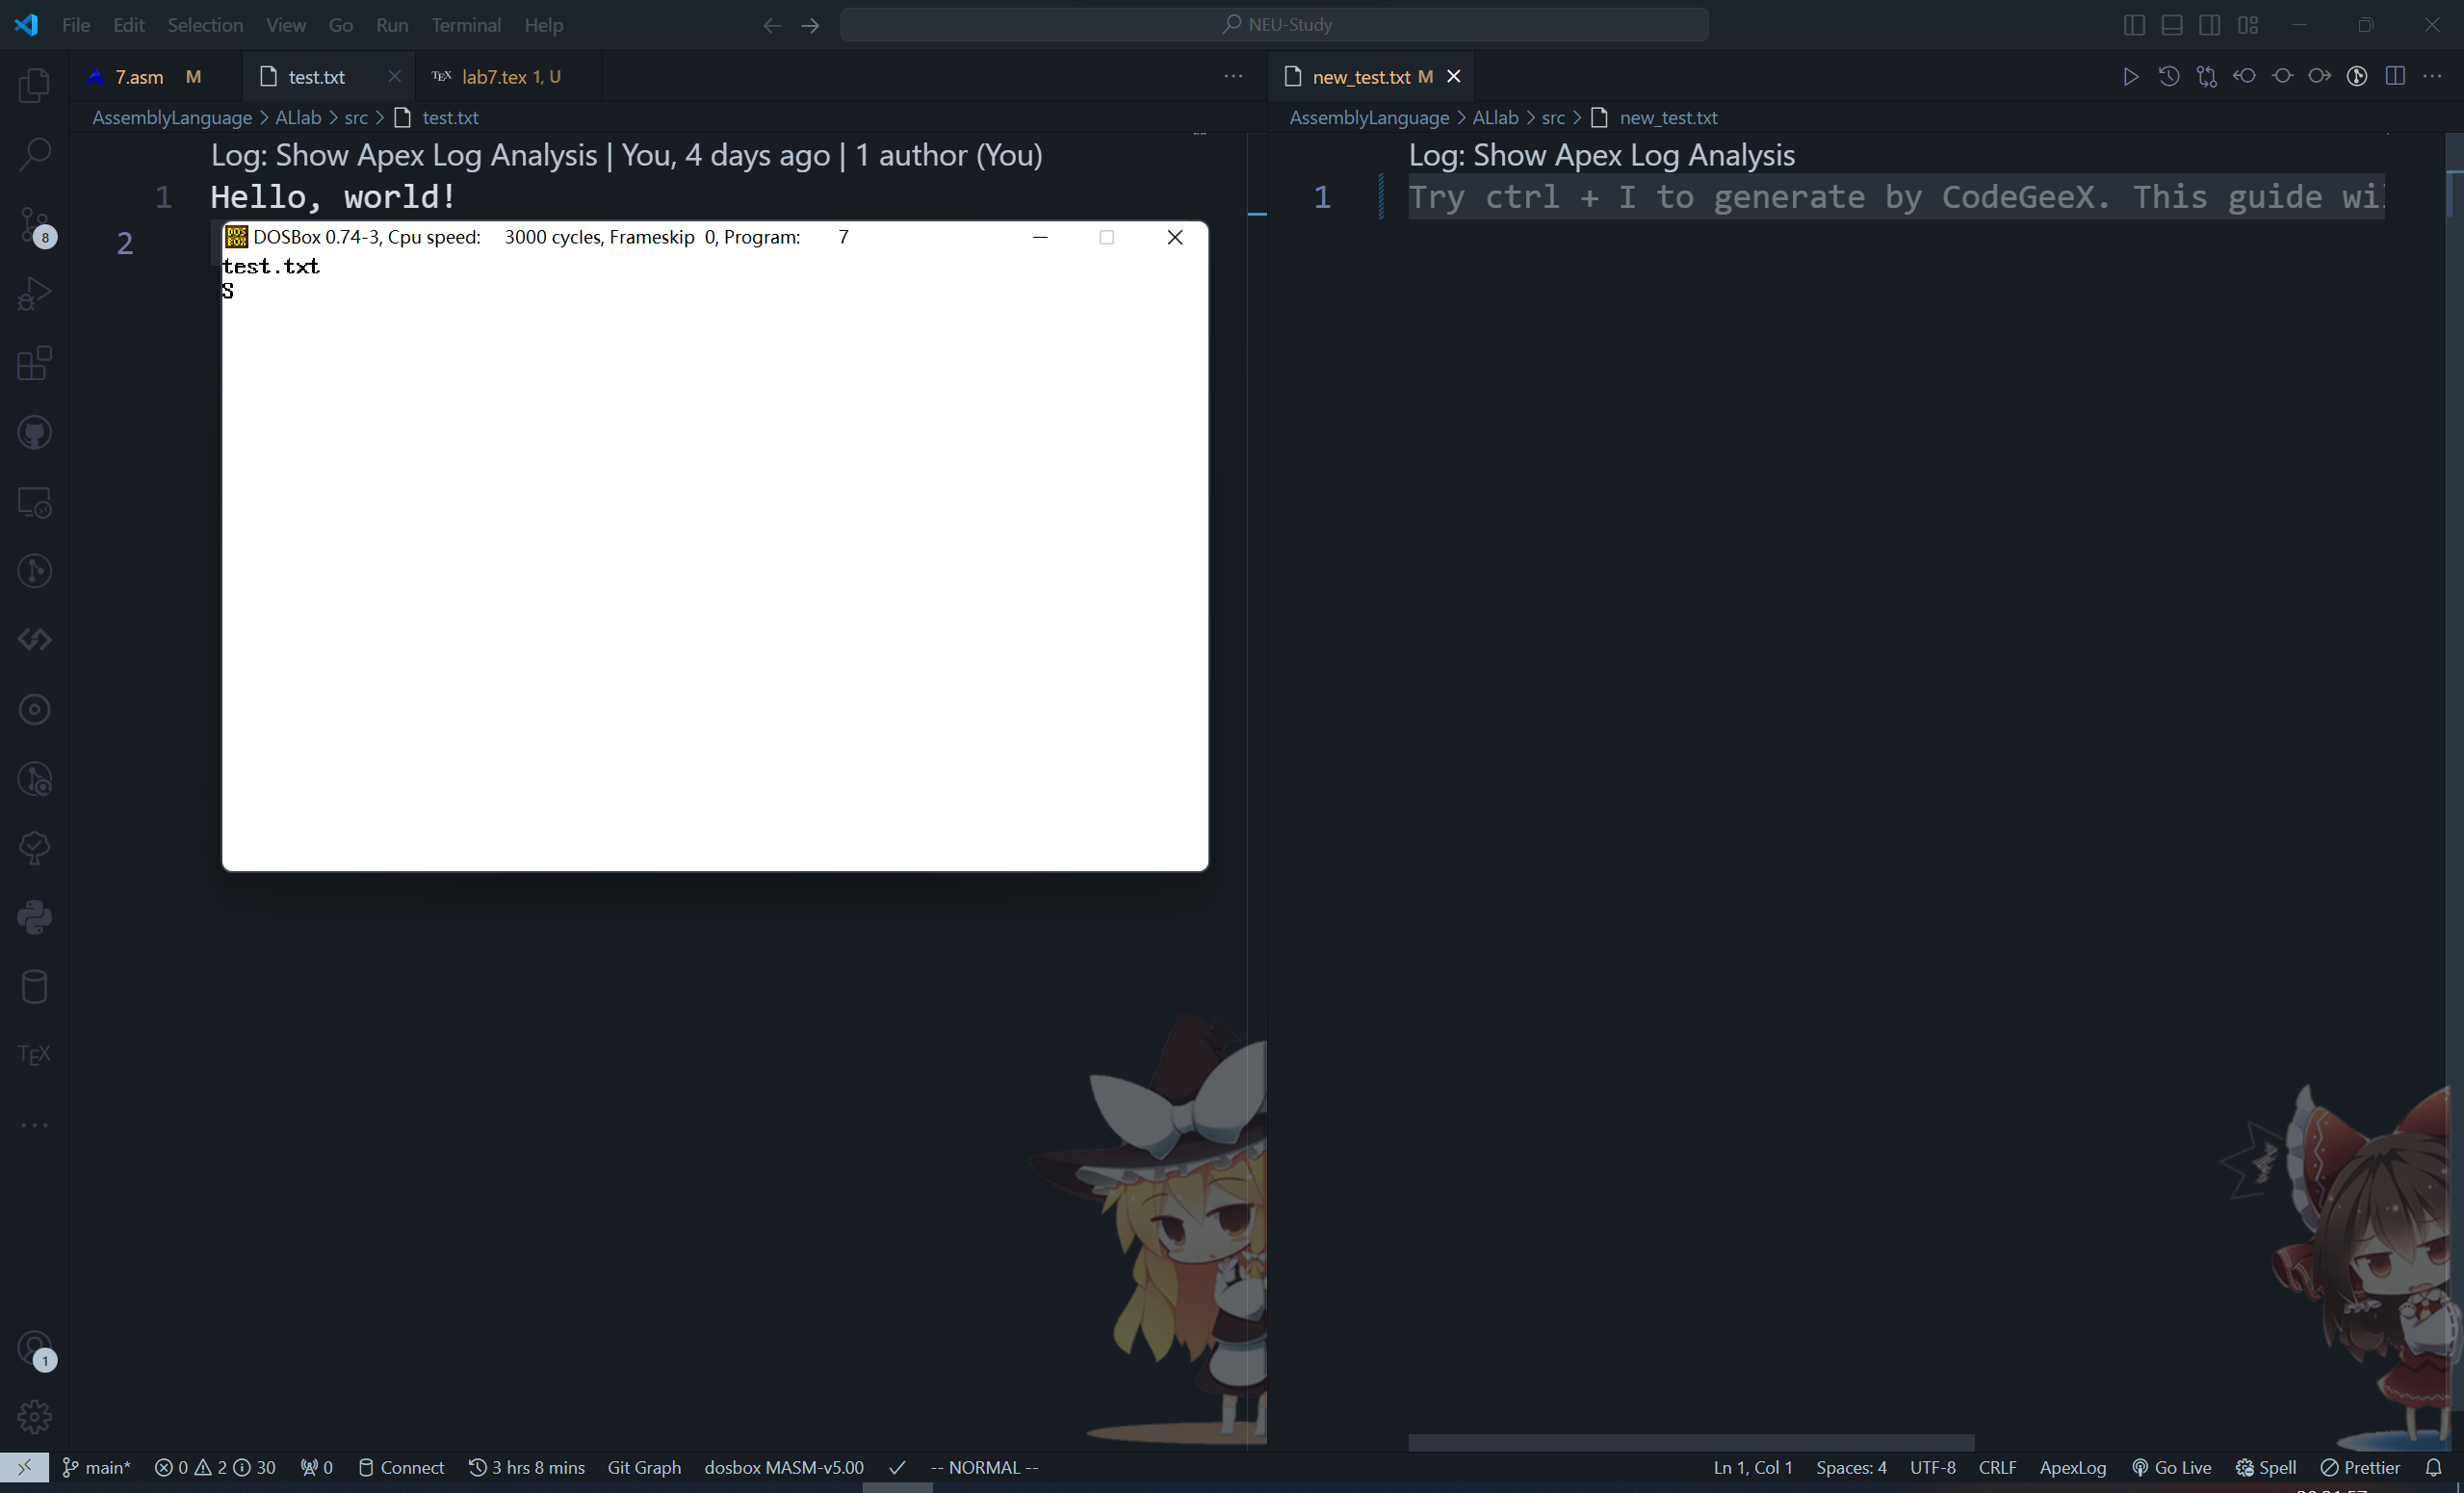
\includegraphics[width=1\textwidth]{image/AL_65.png}\end{center}
    输出文件
    
    \begin{center}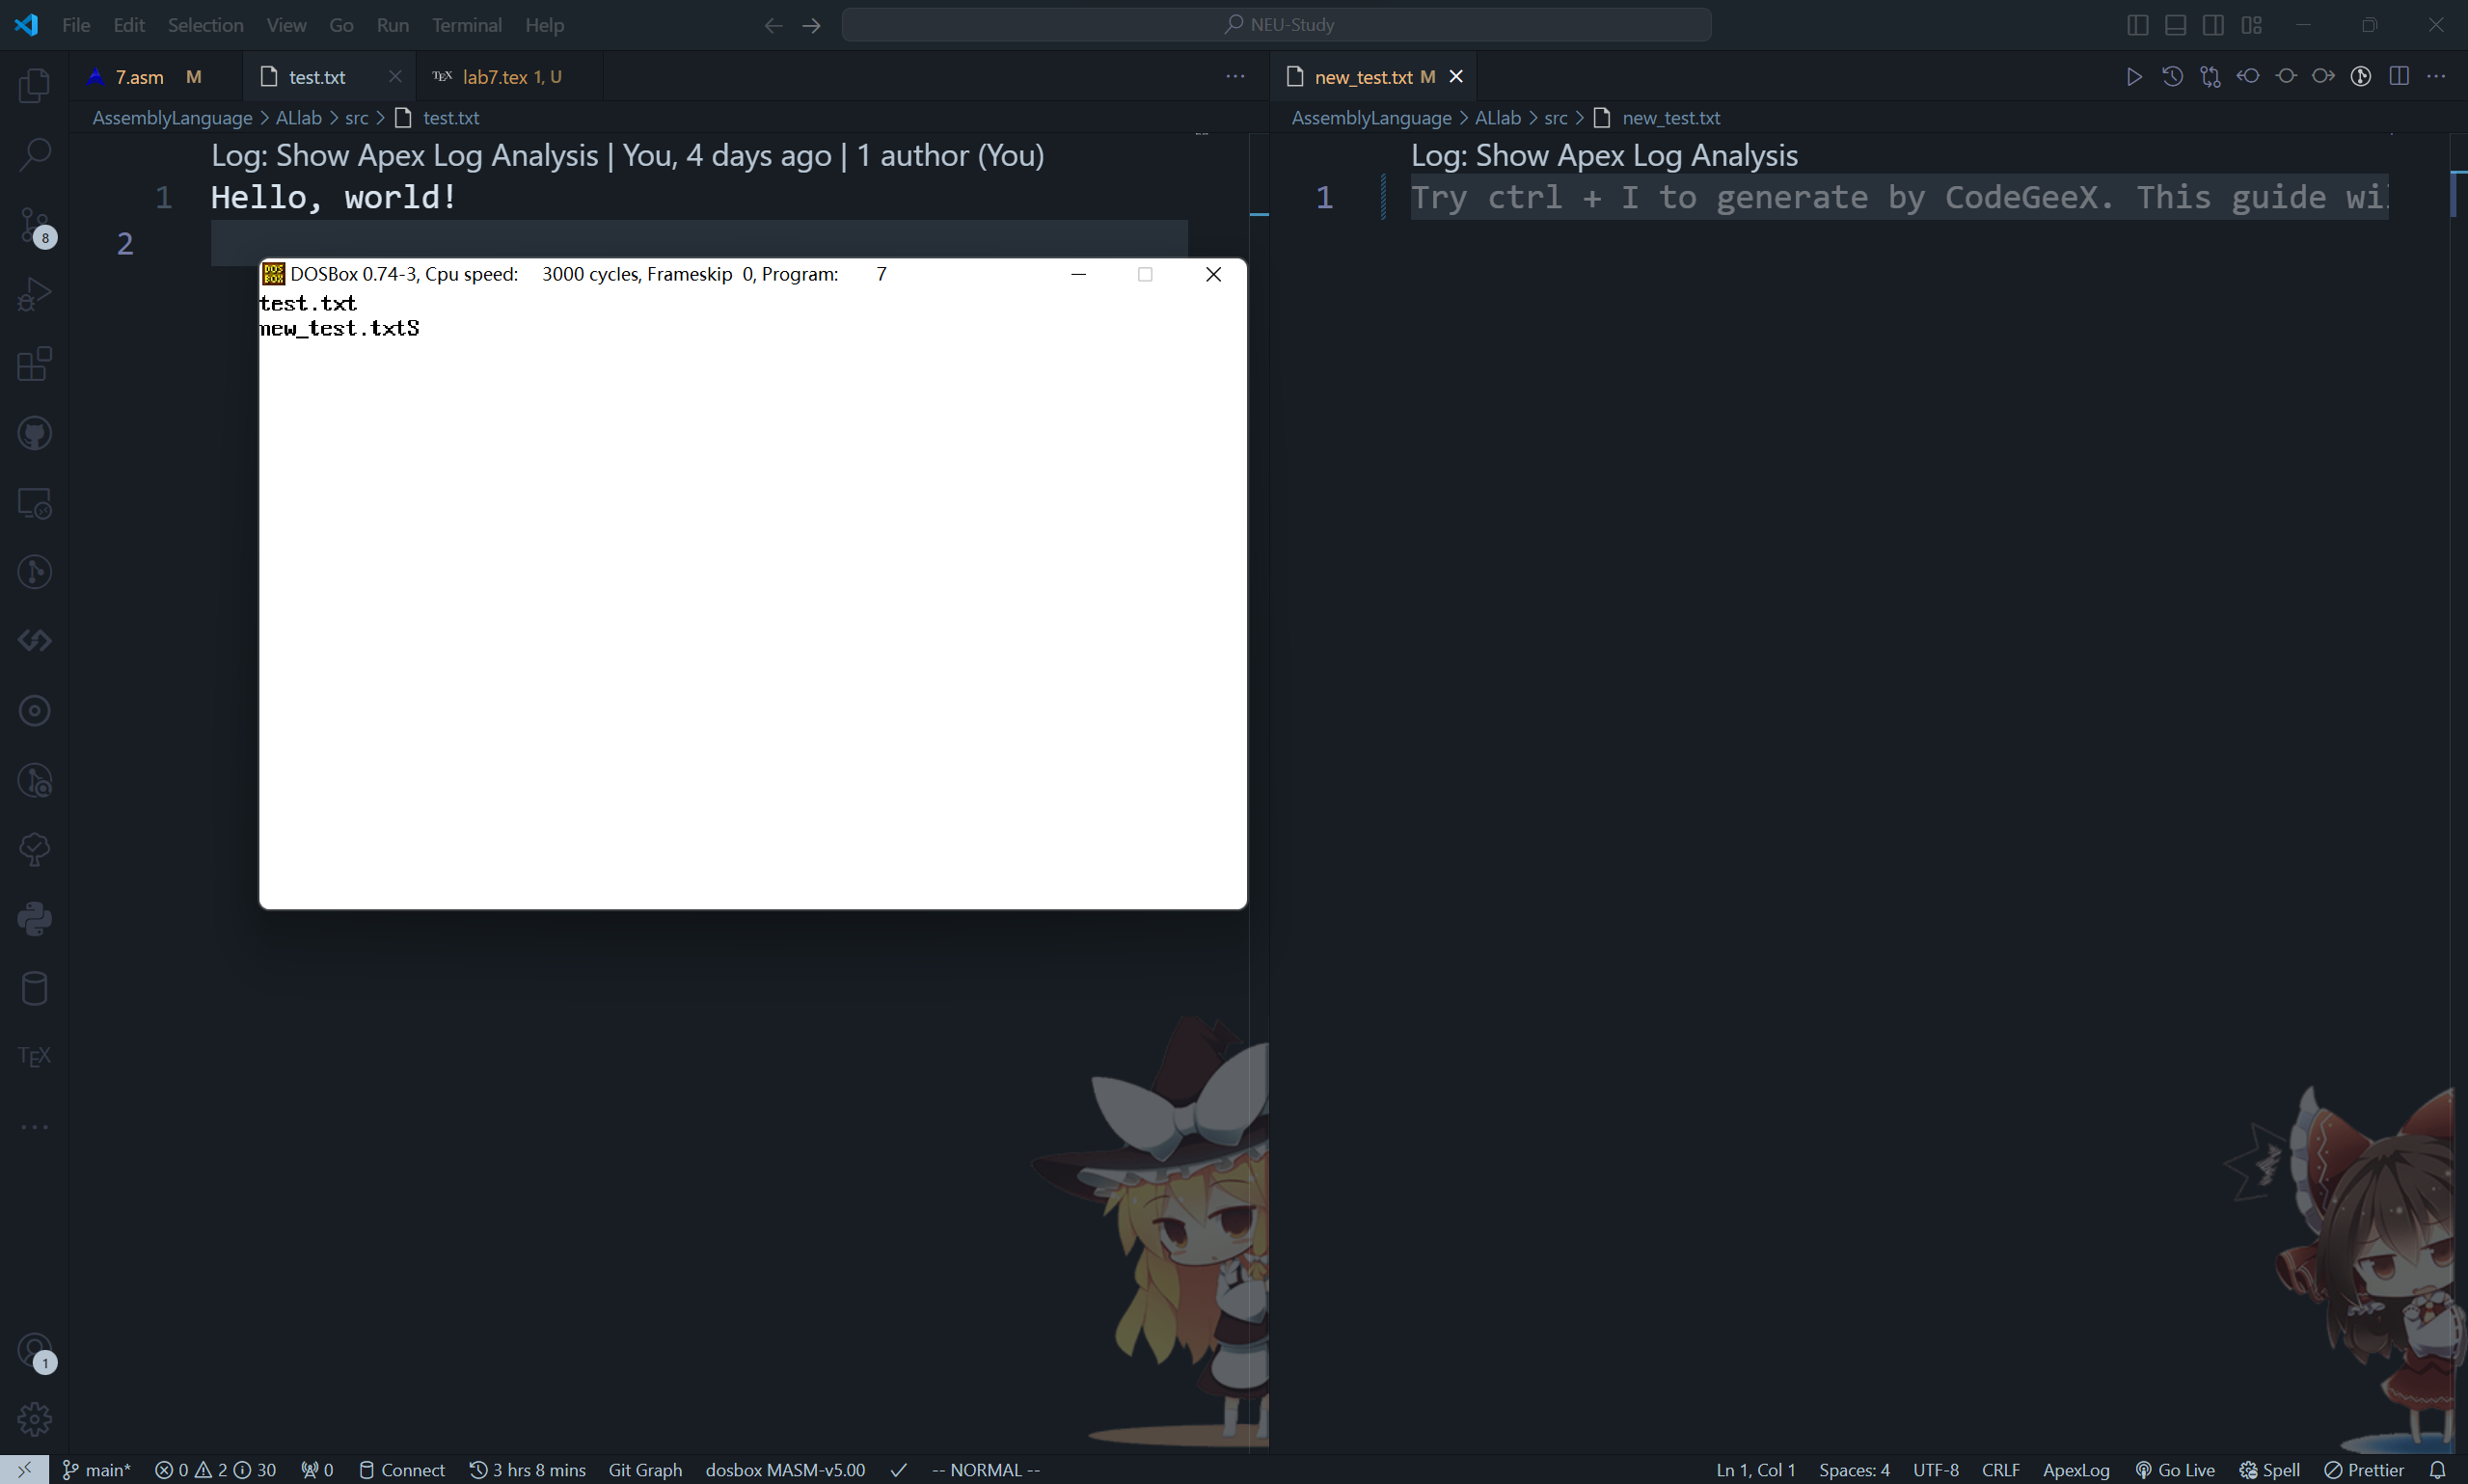
\includegraphics[width=1\textwidth]{image/AL_66.png}\end{center}
    \begin{center}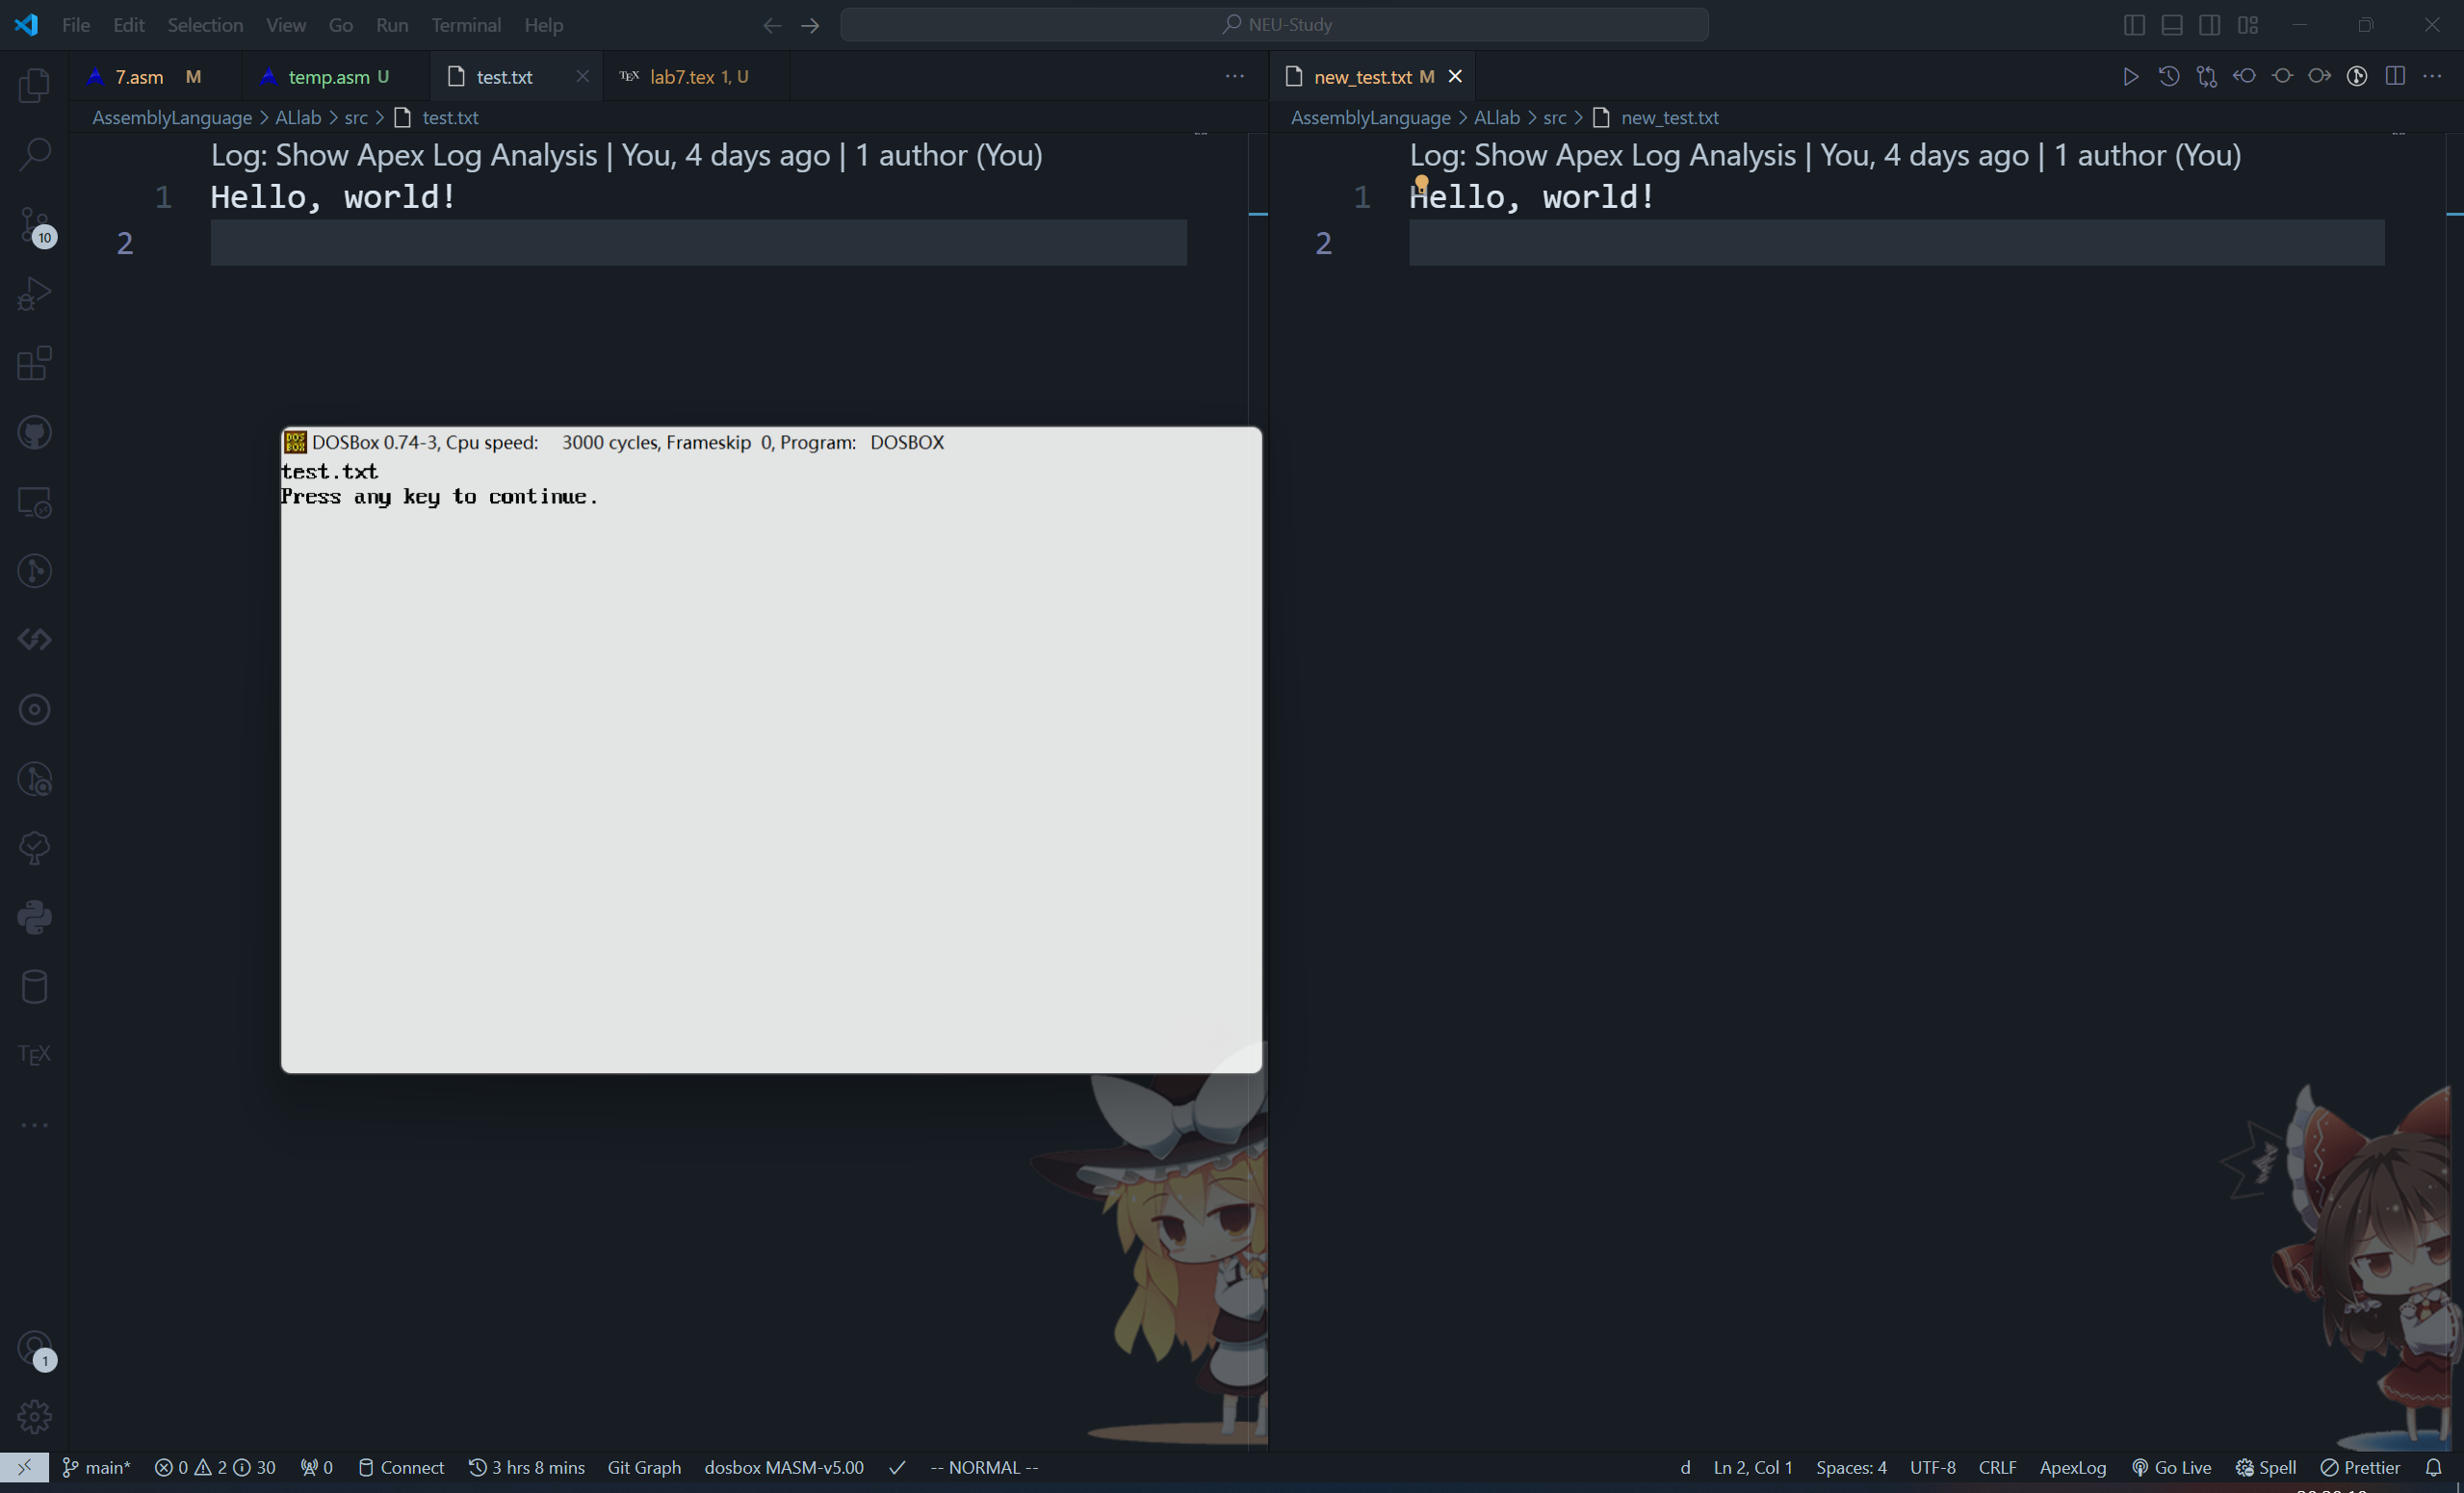
\includegraphics[width=1\textwidth]{image/AL_67.png}\end{center}

    \subsection{流程图}
    \begin{center}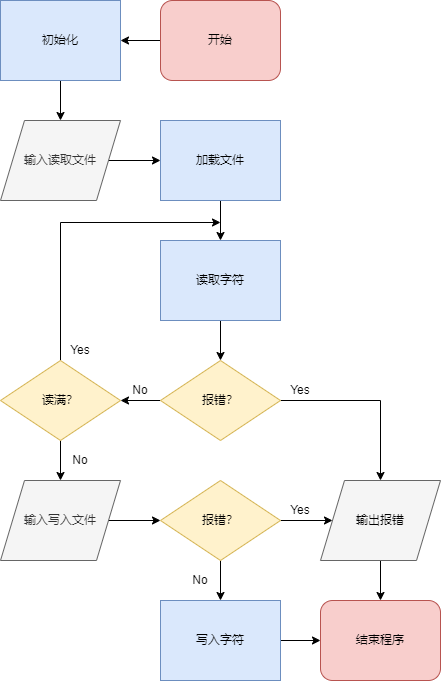
\includegraphics[width=0.5\textwidth]{image/AL_68.png}\end{center}

\section{心得体会}
通过完成这次的文件复制实验，我对汇编语言在实际应用中的功能有了更深入的理解。
实验不仅加强了我对BIOS和DOS中断调用的知识，也让我更熟练地掌握了文件操作的基本技巧。

我学到了如何使用DOS中断来处理文件，包括如何打开、读取、写入和关闭文件。
通过直接与操作系统的底层交互，我对操作系统如何管理文件和设备有了更清晰的认识。
这种底层的编程能力是高级语言难以提供的，它让我能更精确地控制程序的行为。

在实验过程中，我遇到了几个技术挑战，其中最大的挑战是正确处理文件的读取和写入。
最初，我发现复制出来的文件无法正确打开，后来通过调试发现是因为文件句柄没有正确管理。
我通过阅读DOS中断的文档并咨询教师，学习到了如何正确地处理文件句柄和确保文件结束标志正确设置的方法。

此外，我还遇到了文件名输入错误导致的问题。
在用户输入错误的文件名时，程序需要有鲁棒的错误处理机制来给出清晰的错误提示。
通过增加输入验证的逻辑，我学会了如何使程序能更友好地与用户交互，并提高了程序的用户体验。

通过解决这些问题，我不仅提升了自己的编程技能，也增强了解决问题的能力。
我学会了如何在程序中实现更复杂的逻辑控制，以及如何通过程序代码直接与硬件和操作系统交互。

这次实验不仅让我掌握了汇编语言编程的实用技能，也让我认识到了在程序设计和开发中细节的重要性。
每一次的编程实践都是对我理论知识的深化和技能的锻炼，我期待将这些知识应用到未来更复杂的项目中，以解决更具挑战性的问题。

\begin{flushright}\begin{tabular}{rl}
    姓名: & 李俊洁\\
    班级: & 计算机2204 \\
    学号: & 20225443 \\
    课程: & 汇编语言程序设计 \\
    日期: & April 24, 2024 \\
    制作: & \LaTeX \\
    & 感谢您的批阅！
\end{tabular}\end{flushright}
\end{document}